\subsubsection{Venue : Creating new venue}
	Once a user has been successfully authenticated by the UPRM system, the user should be able to create a new venue. The venue creation will require the following information before the creation is finalised: 
	\begin{itemize}
		\item Name of the new venue.
		\item The name of the organisation responsible for the venue.
		\item A date signifying the deadline for submissions.
		\item Contact details to where the submissions should be posted (i.e. email address).
	\end{itemize}
	\textbf{Pre-Conditions}
	\begin{itemize}
		\item User has to be successfully authenticated.
	\end{itemize}
	\textbf{Post-Conditions}
	\begin{itemize}
		\item A new venue should be created.
		\item The new venue information should be saved in a database.
	\end{itemize}
	\textbf{Use case diagram for creation of venues: }\\
	\centerline{\fbox{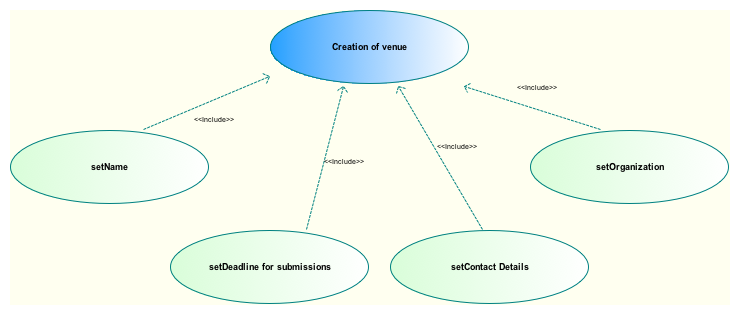
\includegraphics[width=\linewidth]{venue/uprm_venueCreate.png}}}